% Optional insertions; do not duplicate main figures already included by chapter6.

\begin{figure*}[t]
\centering
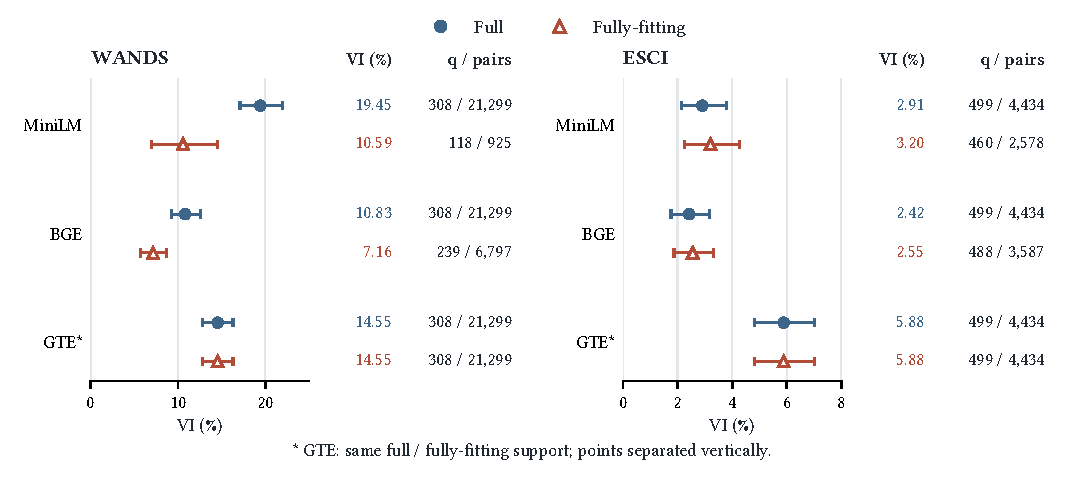
\includegraphics[width=\textwidth]{figures/rq1_vi_top20_main.pdf}
\caption{At K=20, dots and triangles show query-macro VI for full and fully-fitting highest-relevance target populations, respectively. VI is the fraction of targets whose inclusion crosses the cutoff within the seven-order family, averaged within query and then across eligible queries. Fitting requires every complete serialized input, including special tokens, to fit under all seven schedules at that encoder's cap (MiniLM 256, BGE 512, GTE 8192). The full raw C0 competitor catalog is fixed: 42,994 WANDS or 10,076 ESCI products before target replacement. Non-fitting competitors are retained. Each target is replaced independently in its own index. Values and q/pair denominators appear beside every point. GTE full and fitting supports coincide, so identical estimates and intervals are separated vertically. The WANDS and ESCI panels use different horizontal ranges. Differences between full and fitting populations are descriptive, not causal truncation effects. Encoder-specific fitting supports differ; these comparisons do not identify intrinsic cross-encoder sensitivity. WANDS uses 308 eligible queries and 21,299 Exact pairs from its existing held-out split (384 requested queries). ESCI uses 499 eligible queries and 4,434 E pairs from its existing 500-query evaluation sample, not a newly held-out sample. Intervals reuse the existing 95\% paired query-cluster percentile bootstrap endpoints (10,000 draws; seed 2026091701). Products and comparisons from a sampled query remain together. Intervals are descriptive and uncorrected for multiple comparisons; inclusion of zero does not establish equivalence.}
\Description{Two panels show Top-20 VI with horizontal 95\% intervals for WANDS and ESCI, each with MiniLM, BGE, and GTE. Filled circles denote full targets, open triangles fully-fitting targets. Each estimate has a numeric VI percentage and query/pair count. Full/fitting VI percentages are WANDS MiniLM 19.45/10.59, BGE 10.83/7.16, GTE 14.55/14.55; ESCI MiniLM 2.91/3.20, BGE 2.42/2.55, GTE 5.88/5.88. GTE points are separated vertically despite identical support and intervals. All competitors remain raw C0.}
\end{figure*}

\begin{figure*}[t]
\centering
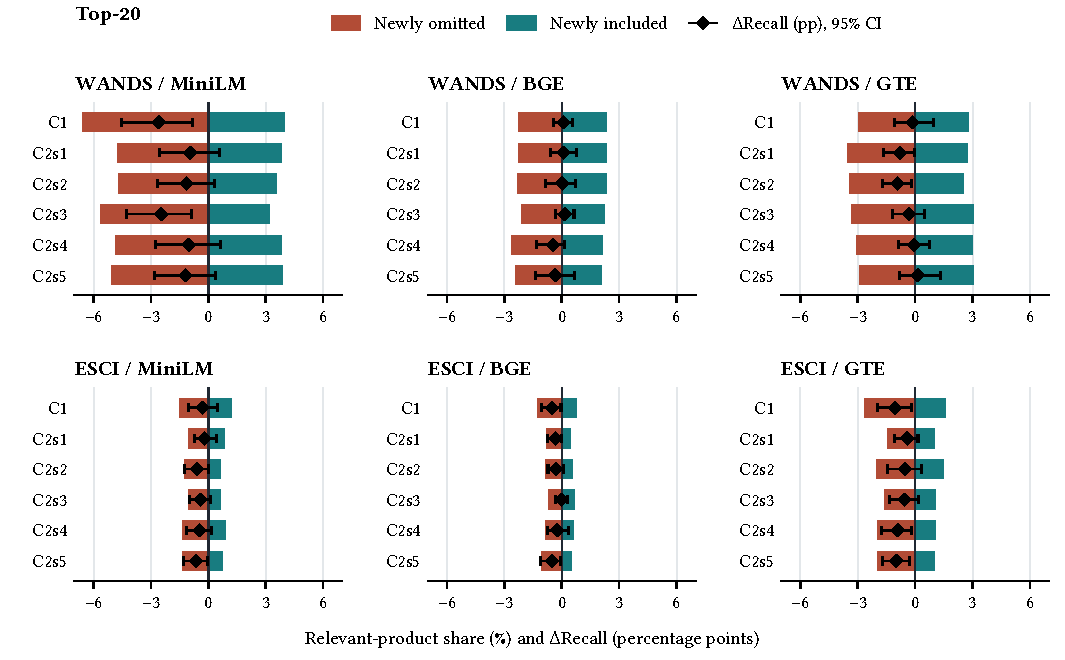
\includegraphics[width=\textwidth]{figures/rq2_membership_top20_main.pdf}
\caption{Catalog-wide membership changes relative to source order at K=20. Left/right bars are newly omitted/included fractions of each complete Hq, averaged across queries. Diamonds and 95\% paired intervals are net Recall. All six comparisons and six panels are retained; values and intervals are unchanged from the historical figure.}
\Description{Six panels show WANDS and ESCI with MiniLM, BGE and GTE. Newly omitted shares extend left and newly included shares extend right of zero. Black diamonds and intervals represent net Recall. C1 and five random schedules are each compared with C0. Interval bars do not describe the colored bars.}
\end{figure*}

\begin{figure*}[t]
\centering
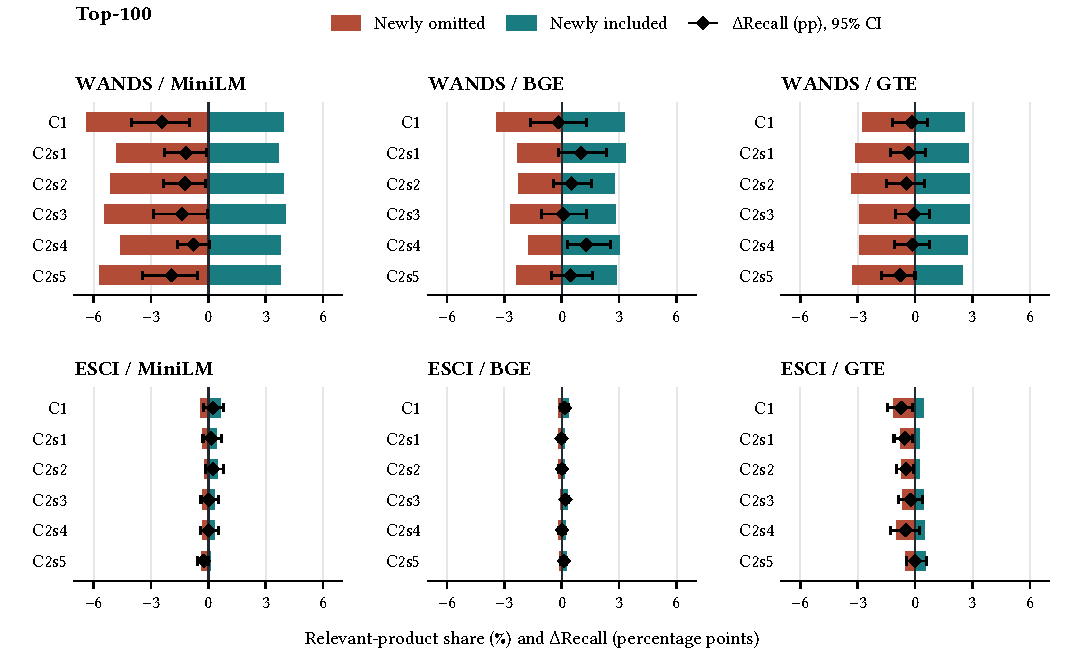
\includegraphics[width=\textwidth]{figures/rq2_membership_top100_appendix.pdf}
\caption{Catalog-wide membership changes relative to source order at K=100. Left/right bars are newly omitted/included fractions of each complete Hq, averaged across queries. Diamonds and 95\% paired intervals are net Recall. All six comparisons and six panels are retained; values and intervals are unchanged from the historical figure.}
\Description{Six panels show WANDS and ESCI with MiniLM, BGE and GTE. Newly omitted shares extend left and newly included shares extend right of zero. Black diamonds and intervals represent net Recall. C1 and five random schedules are each compared with C0. Interval bars do not describe the colored bars.}
\end{figure*}

\begin{figure*}[t]
\centering
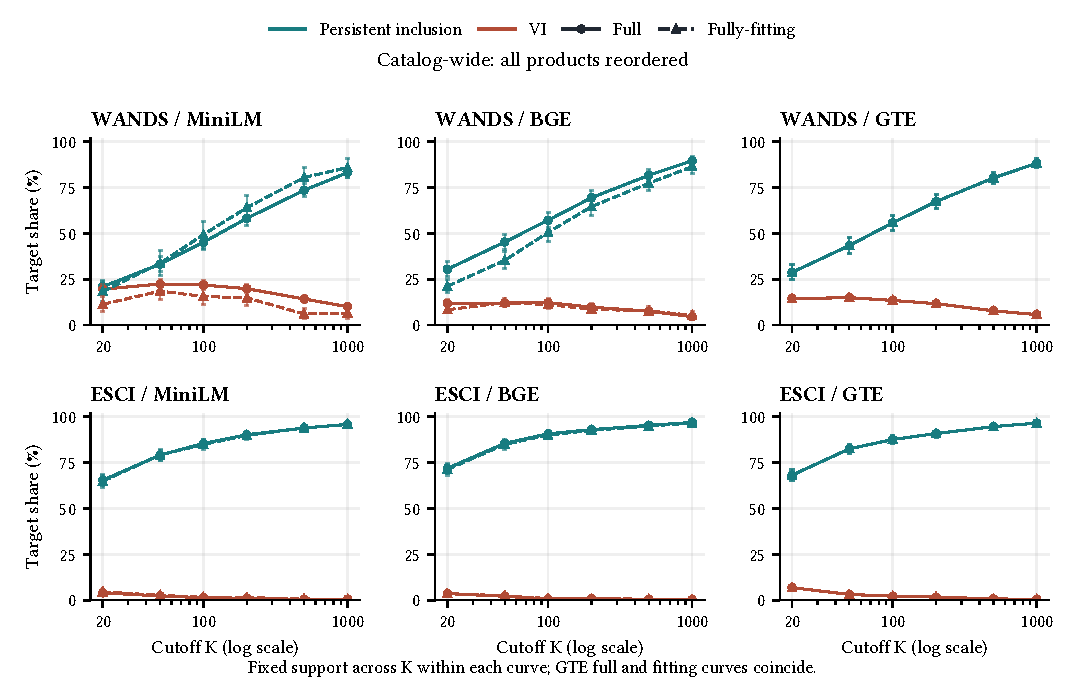
\includegraphics[width=\textwidth]{figures/cutoff_catalog_wide_appendix.pdf}
\caption{catalog-wide cutoff sensitivity at K=20,50,100,200,500,1000. Query-macro persistent inclusion and VI use fixed full or encoder-specific fully-fitting targets and complete unchanged competitor catalogs. Error bars are 95\% query-cluster intervals with common paired resamples. Persistent omission and paired cutoff changes are in the data tables. VI need not decrease with K.}
\Description{Six panels compare full solid curves and fully-fitting dashed curves for WANDS and ESCI and three encoders. Green curves show persistent inclusion and rust curves show VI. Cutoffs are on a logarithmic horizontal axis. Full and fitting GTE curves overlap. The target-only curves describe separate counterfactual indexes, not Recall from one shared index.}
\end{figure*}

\begin{figure*}[t]
\centering
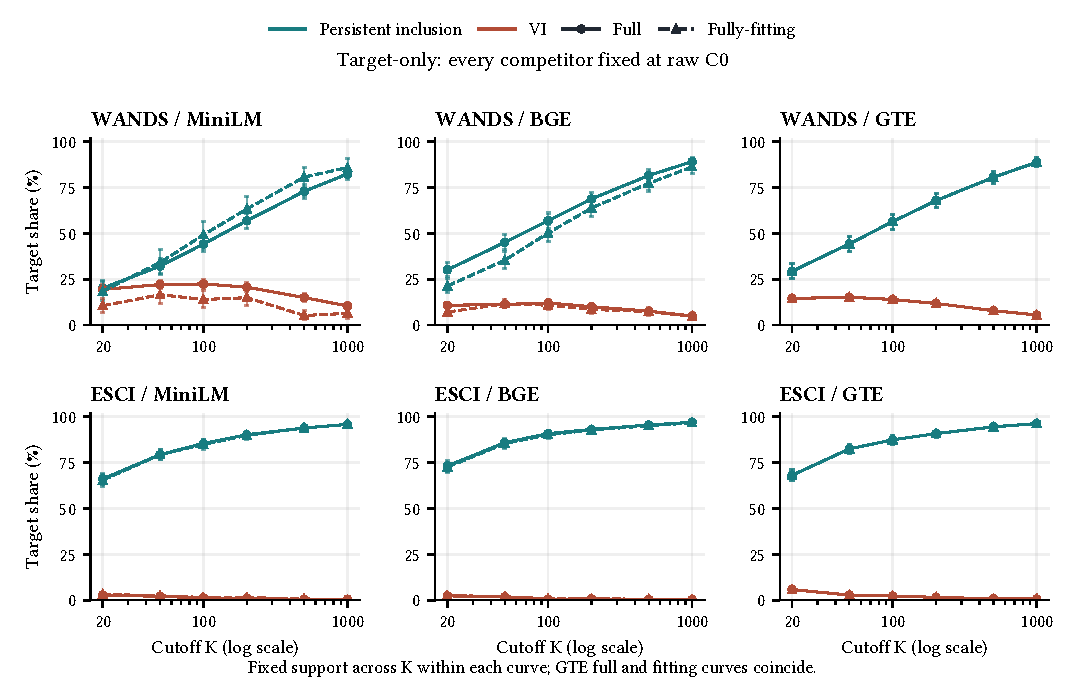
\includegraphics[width=\textwidth]{figures/cutoff_target_only_appendix.pdf}
\caption{target-only cutoff sensitivity at K=20,50,100,200,500,1000. Query-macro persistent inclusion and VI use fixed full or encoder-specific fully-fitting targets and complete unchanged competitor catalogs. Error bars are 95\% query-cluster intervals with common paired resamples. Persistent omission and paired cutoff changes are in the data tables. VI need not decrease with K.}
\Description{Six panels compare full solid curves and fully-fitting dashed curves for WANDS and ESCI and three encoders. Green curves show persistent inclusion and rust curves show VI. Cutoffs are on a logarithmic horizontal axis. Full and fitting GTE curves overlap. The target-only curves describe separate counterfactual indexes, not Recall from one shared index.}
\end{figure*}

\begin{figure*}[t]
\centering
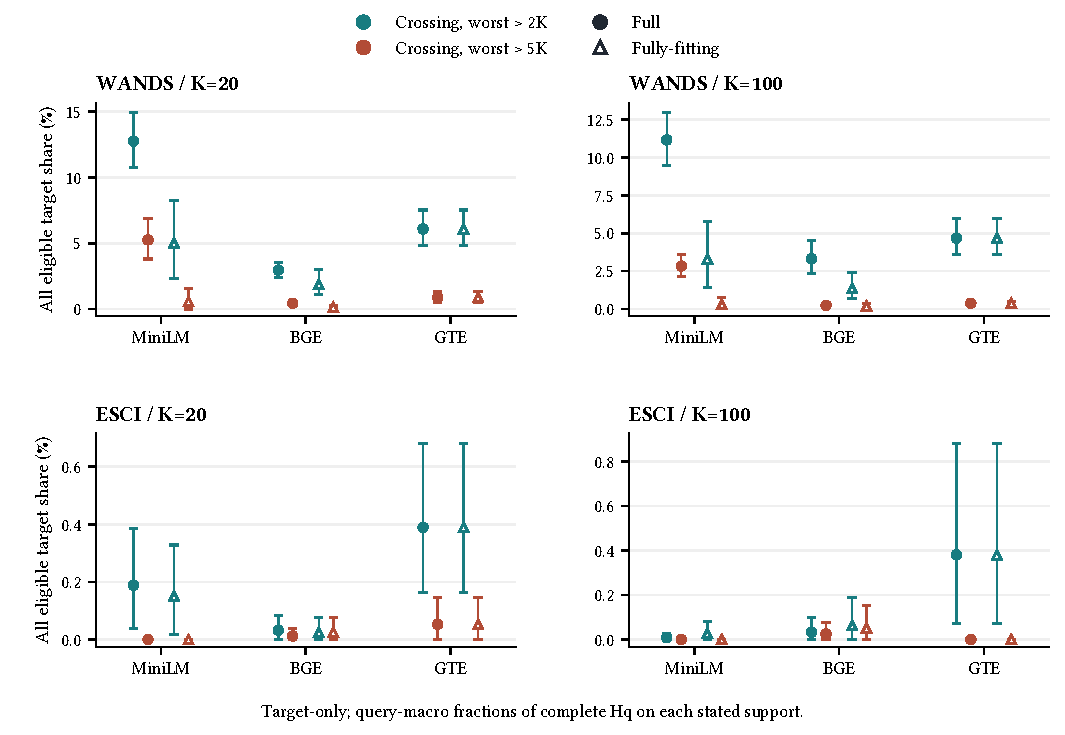
\includegraphics[width=\textwidth]{figures/crossing_severity_appendix.pdf}
\caption{Target-only cutoff crossings with worst rank beyond 2K or 5K. Fractions first divide by all eligible targets within each query, then average queries. Full and fully-fitting supports are separate; competitors are never filtered. Error bars are 95\% paired query-cluster intervals. Conditional crossing-query proportions, pair counts and source-order-directed losses are supplied separately.}
\Description{Four panels cross WANDS and ESCI with K=20 and K=100. Teal points are crossing targets with worst rank above twice K, rust points above five times K. Filled circles denote full targets; open triangles denote fully-fitting targets. Vertical scales differ between panels. Some ESCI estimates are exactly zero.}
\end{figure*}

\begin{figure*}[t]
\centering
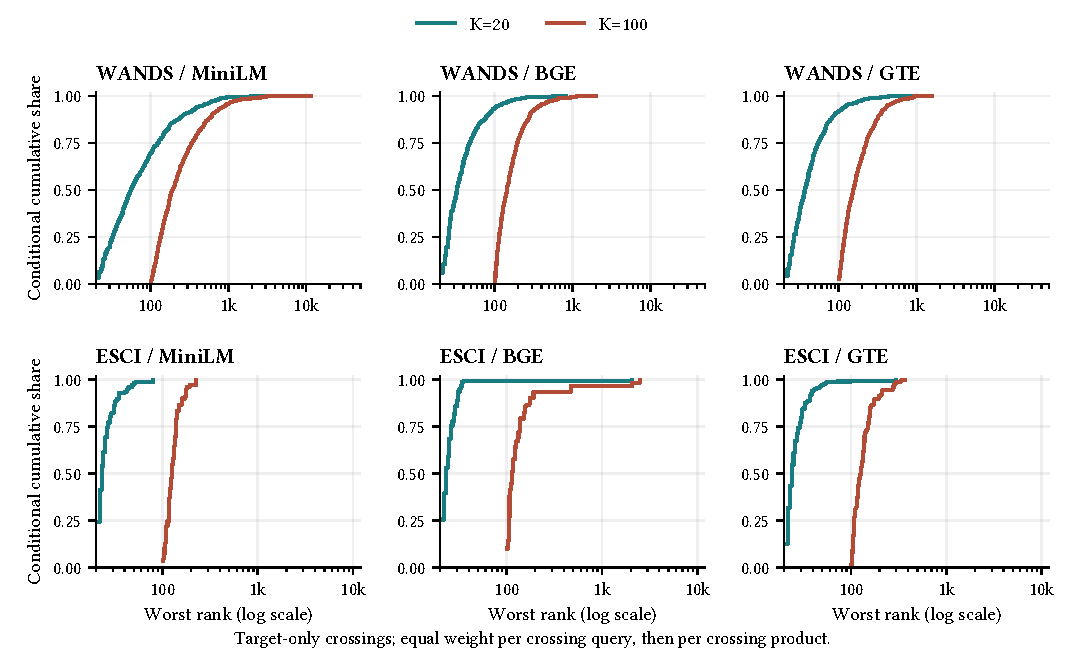
\includegraphics[width=\textwidth]{figures/crossing_worst_rank_ecdf_appendix.pdf}
\caption{Worst-rank ECDF among target-only crossing pairs at K=20 and 100, full primary populations. Crossing means best $\leq$ K < worst. Each query with at least one crossing has equal weight and each crossing product within that query has equal weight. This conditional weighting differs from fractions of all Hq and from pair-micro ECDFs. Fully-fitting and rank-range distributions are in the machine-readable data.}
\Description{Six panels show conditional worst-rank ECDFs for each dataset and encoder. K=20 is teal and K=100 is rust. The horizontal rank scale is logarithmic and panel ranges differ. Curves represent full target supports only, with crossing-query weighting.}
\end{figure*}
